\chapter{Implementering}

Gruppen har lavet en konkret implementering af mønsteret. I det implementerede eksempel kan der vælges mellem forskellige deserilizations-metoder. Implementeringen er lavet så en handler kan formatere XML og JSON format til konkrete klasser. Dette er gjort generisk, således at det er ligegyldigt hvilken type objekt, der skal deserilizeres. 
\\
\noindent Den overordnede abstrakte klasse, som skulle styre chainen ses nedenfor

\begin{lstlisting}
public abstract class ChainHandler<T>
  {
     public ChainHandler<T> NextChain { get; set; }

     public void SetNextChain(ChainHandler<T> nextChain)
     {
         NextChain = nextChain;
     }

     public abstract T Parse(string inputdata, string inputtype);

  }
\end{lstlisting}  

I forhold til beskrivelsen ses det, at nextChain sættes i metoden SetNextChain. Som det kan ses vælges den konkrete handler på baggrund af en streng, her kaldet inputtype. Det væsentlige for de nedarvede klasser er, at alle chainhandlers skal implementere metoden Parse. Metoden skal så, som beskrevet i afsnit Beskrivelse, kalde Parse på NextChain, hvis den ikke selv kan håndtere kaldet, og derigennem kalde den næste i kæden.

\begin{lstlisting}
  class XMLParser<T> : ChainHandler<T>
    {
        public override T Parse(string inputdata, string inputtype)
        {
            if (inputtype.ToLower() == "xml")
            {
                Console.WriteLine("This is xml, I am parsing this");
                var serializer = new XmlSerializer(typeof(T));
                var type = (T) serializer.Deserialize(new StringReader(inputdata));
                return type;
            }
            return NextChain.Parse(inputdata, inputtype);
        }
    }
\end{lstlisting} 

\noindent Ovenfor ses et eksempel på en af handlerne. Som det kan ses nedarves den abstracte Chainhandler. Selve funktionen tjekker på strengen inputtype fortæller om typen er XML. Hvis inputtype er XML, så håndterer denne klasse kaldet, og laver objekter ud fra den streng kaldet inputdata, baseret på en antagelse om at det er XML format. Hvis ikke inputtypen er XML kaldes Parse på Nextchain. Klassen håndtere ikke hvis inputtypen ikke er XML. 

\begin{lstlisting}
//Setup Chain of Responsibility
            ChainHandler<Car> handler1 = new JsonParser<Car>();
            ChainHandler<Car> handler2 = new XMLParser<Car>();
            ChainHandler<Car> handler3 = new TextParser<Car>();

            handler1.SetNextChain(handler2);
            handler2.SetNextChain(handler3);
\end{lstlisting} 
   
\noindent Som det ses ovenfor skal chainen sættes manuelt op i klienten. Handler 1 skal således kaldes for at være sikker på at alle led i kæden bliver traverseret. 

\noindent Det fulde klassediagram, ses på figur \ref{fig:KonkretKlassediagram}. Det kan ses, at det ligner det generelle diagram meget.

\begin{figure}[H]
	\centering
	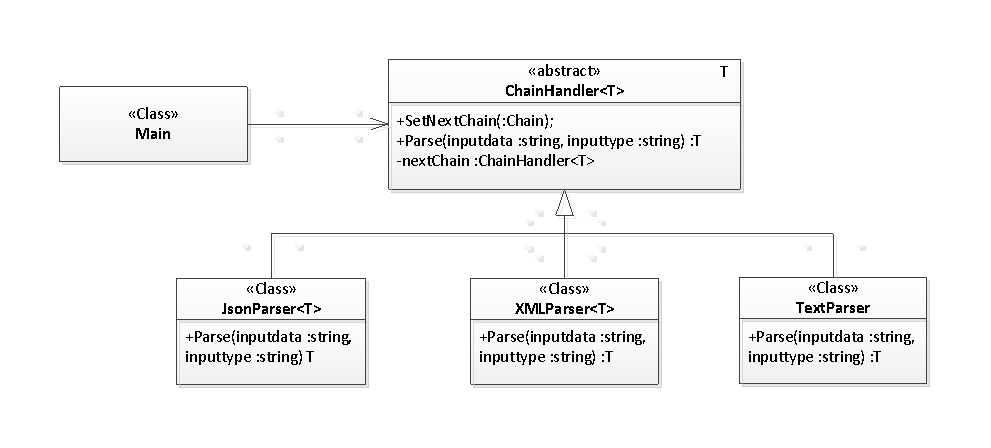
\includegraphics
	[width=140mm]{figures/KonkretUML.pdf}
	\caption{Klassediagram for implementering af Chain of Responsibility}
	\label{fig:KonkretKlassediagram}
\end{figure} 





